\section{Background}
\label{sec: background}
In this section, we offer some background information relevant to our study, focusing on the concurrency control protocols used by the evaluated systems and the important aspects of the PPS workload used in our benchmark.

\subsection{Evaluated Systems}
This study evaluates four database systems that support globally distributed transactions: Detock, SLOG, Calvin, and Janus, using the benchmarking framework we implemented. Each system has its unique deployment strategy and concurrency control approach for handling distributed transactions.

Among these, Detock, SLOG, and Calvin are based on \textit{deterministic scheduling}, an alternative to traditional protocols that use atomic commitment \cite{thomson2010case}. These deterministic database systems avoid the need for runtime coordination between different servers by predefining the execution order of the transactions. This design reduces the communication overhead during transaction execution, which offers notable performance benefits, especially in the presence of inter-region delays. However, this type of locking protocol requires complete knowledge of each transaction's read and write sets in advance. As a result, these systems face challenges when handling \textit{dependent transactions}, namely transactions for which the accessed records are not known beforehand, but must be discovered as the execution progresses.

The three deterministic systems we consider are:
\begin{itemize}
    \item \textbf{Calvin} is the system that demonstrated the practical feasibility of deterministic transaction processing with near-linear scalability \cite{thomson2012calvin}. It is organized into three separate layers. First, the \textit{sequencing layer} receives the transactional requests from the clients, batches them using short epochs, and ensures consistent ordering among the replicas. Then, the \textit{scheduling layer} coordinates the transaction execution by acquiring the locks deterministically according to the defined global order and by passing the transactions to the pool of workers. Finally, the \textit{storage layer} handles the physical data access.
    \item \textbf{SLOG} is built on top of Calvin by optimizing for data locality when used in geo-distributed settings \cite{ren2019slog}. It introduced the notion of \textit{single-home transactions} that access data in a single region, and thus can be processed with very low latency without being passed to the sequencing layer. However, the multi-home transactions still follow Calvin's sequencing model.
    \item \textbf{Detock} is also based on Calvin's architecture, but it removes the need for global ordering by using a deadlock resolution protocol via a \textit{dependency graph} \cite{nguyen2023detock}. This approach allows both single-home and multi-home transactions to be scheduled deterministically at each region. In this way, all participating regions construct independently the same dependency graph, and the transactions can be run locally without the need for cross-region communication once all transaction components have been received.
\end{itemize}

On the other hand, \textbf{Janus} is a generalization of the EPaxos protocol that unifies the concurrency control mechanism (used for transaction consistency) and the consensus protocol (used for replication) into a single layer \cite{mu2016consolidating}. The key idea is that both components work by ensuring that the execution history of the transactions is equivalent to a sequential order, which can be verified by defining a \textit{serialization graph}. Janus can commit and replicate the transactions within a wide-area network round-trip under low contention, and requires at most one additional round-trip in case of conflicts.

We selected these four systems because they all support geo-distributed transactions and share comparable architectural principles, such a deterministic execution and graph-based serialization, which aim to reduce the runtime inter-region communication. Despite these foundational similarities, they have clear differences that make each system more suitable for particular workload characteristics or deployment scenarios. Another important aspect is that the Detock codebase provides a unified implementation of all four systems. So, Calvin, SLOG, and Janus were re-implemented within the Detock framework to share a common storage engine, communication layer, and local consensus protocol \cite{nguyen2023detock}. This shared infrastructure ensures that the performance differences from our evaluation come from each system's core design choices rather than unrelated implementation details.

\subsection{Product-Parts-Supplier Workload}
The Product-Parts-Supplier (PPS) workload is a well-established relational structure that simulates a realistic supply chain management system, capturing the interactions between products, their composing parts, and the suppliers that provide those parts.

PPS has been used as a workload in several popular database benchmarking studies, although typically in a limited capacity. For example, Harding et al.~\cite{harding2017evaluation} utilized the PPS workload primarily in a static manner to evaluate the system scalability by varying only the number of client machines. However, their study did not explore other workload characteristics or deployment configurations. Similarly, Serafini et al.~\cite{serafini2016clay} applied the PPS in their evaluations, but they included only read-only transactions since their goal was to assess the effectiveness of their dynamic partitioning scheme rather than to evaluate the full concurrency behavior of the system.

Our benchmarking framework is built upon a set of concrete tables and transaction types drawn from these previous uses of the PPS workload. Specifically, the schema includes three core entities, \textit{Products}, \textit{Parts}, and \textit{Suppliers}, along with two additional tables that maintain the relationships between them. A product can contain multiple parts, and a part can be a component within multiple products. In the same way, a supplier can provide multiple parts, and a part can be provided by multiple suppliers. Figure~\ref{fig: pps-erd} shows the relational schema of the PPS workload.

\begin{figure}[h]
    \centering
    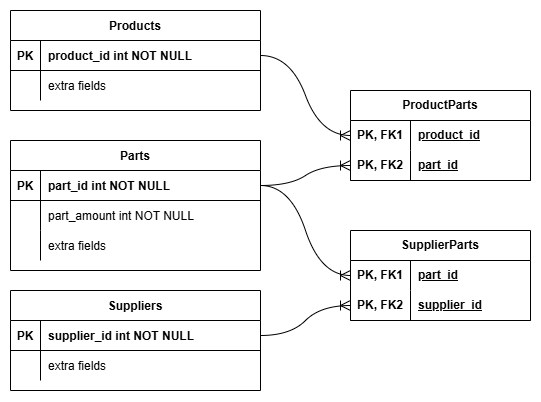
\includegraphics[width=1\linewidth]{figures/PPS ERD.png}
    \caption{Product-Parts-Supplier Entity Relationship Diagram}
    \label{fig: pps-erd}
\end{figure}

The PPS workload has transactions with complex dependencies, which can lead to a significant potential for contention challenges. This complexity makes the workload well-suited to evaluate how database systems handle the coordination and conflict resolution. PPS consists of several types of transactions, including:
\begin{itemize}
    \item \textit{OrderProduct}. Given a $product\_id$, it will first collect the parts associated with the product, and then decrement the inventory amount of these parts. Importantly, this is a dependent transaction, since we don't know which parts will be updated in advance.
    \item \textit{GetPartsByProduct}. Given a $product\_id$, it will retrieve the list of parts associated with the given product.
    \item \textit{UpdateProductPart}. Given $product\_id$, $part\_id\_from$, and $part\_id\_to$, it will modify the first part of the given product to the latter one.
    \item \textit{GetPart}. Given a $part\_id$, it simply fetches the current inventory amount of the given part, along with any existing extra information.
    \item \textit{GetProduct}. Given a $product\_id$, it simply fetches any existing extra information related to the given product.
\end{itemize}